\resetfigpath{eel}
\glsresetall

\chapter{Expected exponential loss for gaze-based video and volume}
\label{eel} % For referencing the chapter elsewhere, use \ref{Chapter1}

\textbf{Author contributions} This chapter combines the contributions of Raphael Sznitman and myself.
Raphael Sznitman contributed on the methodology, coding, and writing of the text.

\textbf{My personal contributions include}:
\begin{itemize}
    \item Discussions on the method.
  \item Providing the data: Videos/Volumes.
    \item Producing manual groundtruth annotations of some of the latter.
    \item Implementing an early prototype of the annotation software eye-gaze tracker
    \item Collecting the point-wise annotations
    \item Producing the superpixel segmentations and optical flow
    \item Producing the deep features
\end{itemize}

\section{Introduction}
Ground truth annotations play a critical role in the development of machine learning methods in medical imaging.
Indeed, advances in deep learning strategies, coupled with the advent of
image data in medicine have greatly improved performances for tasks such as structure detection and anatomical segmentation across most imaging modalities (e.g. MRI, CT, Endoscopy,Microscopy) \cite{kamnitsas17-3d}, \cite{anthimopoulos16}.
Yet the process of acquiring ground truth data or annotations remains
laborious and challenging, especially in video and 3D image data.

To mitigate manual annotation dependence, semi and unsupervised methods have been
key research areas to reduce the overall annotation burden placed on domain experts (e.g. radiologist, biologist, surgeon etc....).
Most notably, \gls{al} \cite{KonSznFua15}, \cite{mosinska16}, \gls{tl} \cite{bermudez16}, \cite{shin16}, and \gls{cs} \cite{maier14}, \cite{cheplygina16}, provide frameworks for learning with either limited or noisy ground truth data and have been applied to a larger number of applications.
Yet in \gls{al} domain experts are still necessary to actively provide ground truth data, sequentially or in batch.
Similarly, \gls{cs} relies on manual annotators to follow carefully crafted labeling tasks in order to leverage non-experts, which produces highly variable ground truth quality \cite{cheplygina16}.

Alternatively, Vilarino et al. \cite{vilarino07} used an eye gaze tracker to annotate polyps in video colonoscopy.
In their approach an expert passively viewed a video and stared at polyps.
From these, they trained an \gls{svm} classifier to label the sequence, treating regions around each gaze location as positives and the rest of the image domain as negative samples.
As we show in our experiments however, this approach is limited to detecting objects of fixed size and does not extend well to pixel-wise segmentation tasks.
Also related is the work in \cite{sadegh09}, which mapped out regions of interest using a gaze tracker on individual frames observed for extended periods of time.
More recently, the work of \cite{khosravan16} is closely related to our setting, with the important distinction that our data is viewed in one pass and applied to video and volumetric data.

To overcome this limitation, we propose a novel framework to produce pixel-wise segmentation for an object present in a volume (or video sequence) using gaze observations collected from a $200\$$ off-the-shelf gaze tracker.
Assuming a single target is present throughout the image data, we cast our problem as a semi-supervised problem where samples are either labeled as positive (gazed image locations) or unknown (the rest of the image data which could be positive or negative).
To learn in this regime, we introduce a new Expected Exponential loss
function that can be used within a traditional gradient boosting framework.
In particular, the expectation is taken with respect to the unknown labels, requiring a label probability estimate.
We describe how to estimate these with a novel strategy and show that our approach not only provides superior performances over existing methods in a variety of medical imaging modalities (i.e. laparoscopy, microscopy, CT and MRI) but can be used in a \gls{cs} context as well.

\section{Gaze-based pixelwise annotation}
Our goal is to produce a pixel-wise segmentation of a specific structure of interest located in a video or in a volume (i.e. we treat a volume as a video sequence).
To do this, we ask a domain expert to watch and follow the structure throughout the sequence.
While viewing the sequence, we track the persons eye gaze by means of a commercially available eye gaze tracker.
In our setting, this provides a single gaze location for each viewed image and we assume the observer is compliant in the task.

To produce ground truth annotations, we cast this problem as a binary semi-supervised
machine learning problem, where one must determine a pixel-wise segmentation of the structure of interest in each of the images using only the sequence itself and the gaze locations.
We assume that gaze locations correspond to the structure and propose a novel Expected Exponential loss function that explicitly takes into account that some labels are known while others are not.
This loss leverages probability estimates regarding the unknown labels and we present a strategy to estimate these effectively.
Note that, we do not focus on learning a function that generalizes to other similar sequences, but one that annotates the given sequence as well as possible.

For a given image sequence, our approach is organized as follows and is illustrated in Fig. \ref{fig:eel_pipeline}:
(1) the expert views the sequence and 2D gaze locations are collected; (2) we estimate the label
probability by using the image data and the gaze information; (3) we then train a gradient
boosted classifier with our proposed loss on a subset of the image data; (4) using the trained
classifier, we predict the remainder of the image data. We will detail these steps in the following
sections but first define some notation used throughout this paper.

\begin{figure}[h]
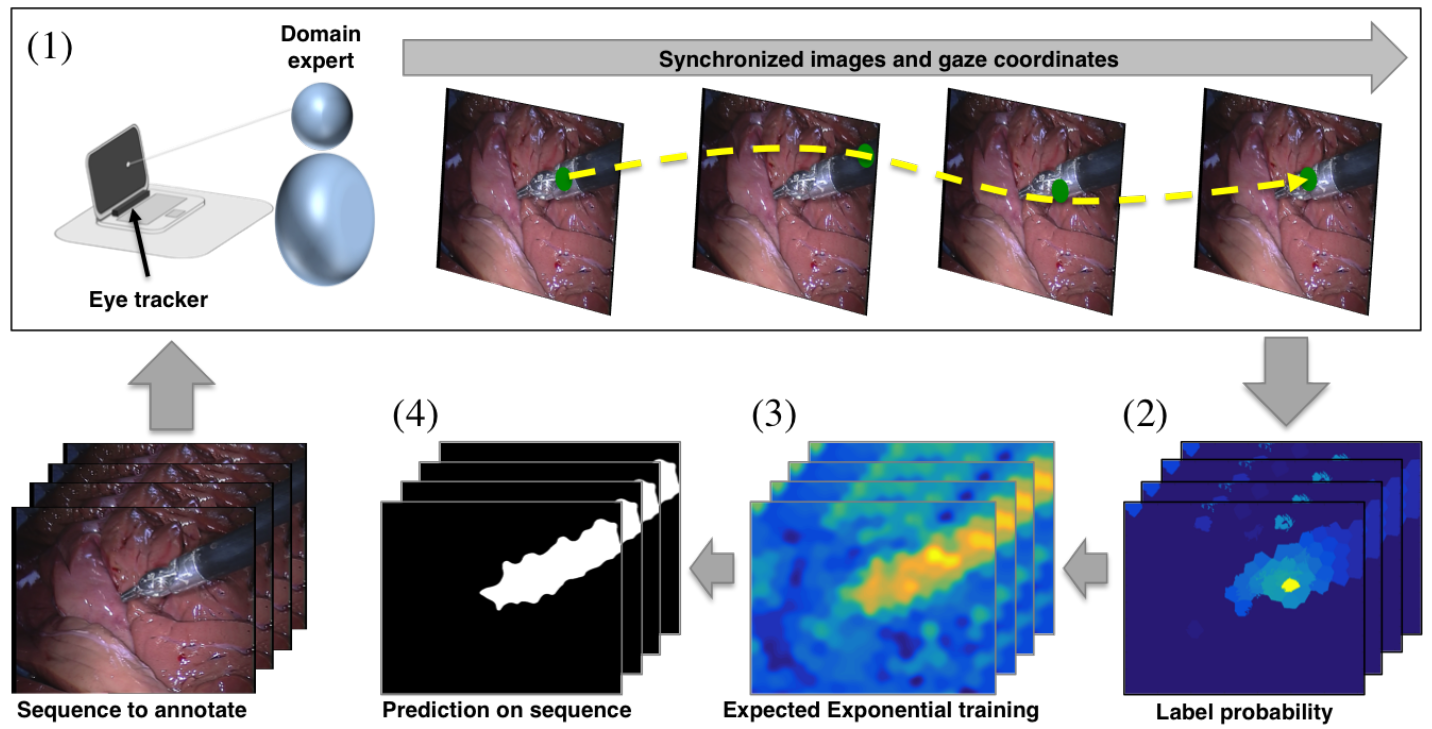
\includegraphics[width=0.99\textwidth]{pipeline}
\caption{Example Gaze-based annotation.
  A surgical instrument must be annotated in a sequence.
  (1) A domain expert watches the sequences and has their gaze collected during the
  viewing.
  (2) Our method then estimates object likelihoods over the sequence and (3) we then
train a classifier with an Expected Exponential loss function using a subset of the image data.
(4) The classifier is then used to evaluate the remainder of the sequence.}
\label{fig:eel_pipeline}
\end{figure}

\section{Notation}
Let an image sequence (or volume) be denoted $\mathcal{I} = [I_{0}, \cdots , I_{T}]$ and let $\mathcal{G} = \{g_{t} \}^{T}_{t=0}$ such that $g_t\in \mathbb{R}^{2}$ is a 2D gaze pixel location in $I_{t}$.

While we ideally would like
a pixel-wise segmentation, we choose to decompose each image using a temporal superpixel
strategy \cite{chang13} and operate at a superpixel level instead.

We thus let $I_t$ be described by the set of non-overlapping superpixels
$S_{t} = \{S^{n}_t\}^{N_t}_{n=0}$ and define the set of all superpixels across all
images as $\mathcal{S} = \{S_t \}^{T}_{t=0}$.
We denote the set $\mathcal{P} = \{S^{n}_t | g_{t} \subset S^{n}_t, t = 0, \cdots, T, n = 0, \cdots, N_t \}$ as all
superpixels observed and the rest as $\mathcal{U} = \mathcal{S} \backslash \mathcal{P}$.
We associate with each $S^{n}_t$ a binary random variable $Y^{n}_{t} \in \{-1, 1\} = \mathcal{Y}$,
such that $Y^{n}_t = 1$ if $S^{n}_t$ is part of the object and -1 otherwise.
In particular, we defined $Y_n$ as a Bernoulli random variable, $Y^{n}_t \sim Ber(\epsilon_{S^{n}_{t}})$, $\epsilon \in (0,1)$.
Note that for positive superpixels $S^{n}_t \in \mathcal{P}$, we consider these as part of the object and let $Y^{n}_t = 1$ with $\epsilon_{S^{n}_{t}}=1$.

\section{Method}
Our goal is to train a prediction function, $f : S \rightarrow Y$
that takes into account observed superpixels as well as the unobserved ones.
To do this we propose the following Expected Exponential Loss (EEL) function:

\begin{equation}
  \mathcal{L}_{EEL} = \mathbb{E}^{Y} \left[ \sum_{S \in \{ \mathcal{P}, \mathcal{U}\}} e^{-f(S)Y}\right]
\end{equation}

where the expectation is taken with respect to all $Y$s.
By linearity of expectation and the fact that labeled superpixels have no uncertainty in their label, we can rewrite the loss for all superpixels as

\begin{equation}
  \label{eq:eel}
  \mathcal{L}_{EEL} = \sum_{S \in \mathcal{P}} e^{-f(S)} + \left( \sum_{S \in \{ \mathcal{P}} \epsilon_{S} e^{-f(S)Y} + (1-\epsilon_{S}) e^{f(S)Y}\right)
\end{equation}

Note that Eq. \ref{eq:eel} is a generalization of the Exponential Loss (EL) \cite{hastie09}.
In the case where labels are known, the loss is the same as the traditional loss as the expectation is superfluous.
For unknown samples, the value of $\epsilon_{S}$ weighs the impact of the superpixels.
For instance, if $\epsilon_{S}$ is close to 0.5, the sample does not affect the loss.
Conversely values of $\epsilon_{S}$ close to 1 (or 0) will strongly impact the loss.

\section{Implementation}
We implemented the above EEL within a traditional Gradient Boosting classifier \cite{hastie09},
by regressing to the residual given by the derivate of Eq. \ref{eq:eel}.
For all experiments, we used stumps as weak learners, a shrinkage factor of 1 and the line search was replaced by a constant weight of 1.
The weak learner stumps operate on features extracted from the center of the superpixel.
In particular, we used generic Overfeat features \cite{sermanet13} which provide a rich
characterization of a region and its context (e.g. 4086 sized feature vector).
During training we used all superpixels in $\mathcal{P}$ and used $10\%$ of those in U.
A total of 50 boosting rounds was performed in all cases.
To predict segmentations for the entire volume, we
predicted the remaining $90\%$ of superpixels in $\mathcal{U}$.

\section{Probability estimation for unknown labels}
\label{sec:eel_estim}
To estimate $\epsilon_{S}$ in Eq. \ref{eq:eel}, we take inspiration from the Label Propagation method \cite{zhou04}, which uses a limited number of positive and negative samples to iteratively propagate labels to unobserved samples.
In our setting however, we only propagate positive samples to unlabeled
samples using the gaze information as well as pixel motion estimation to constrain the probability diffusion.
We let $P_{0} = \left[p_0,\cdots, p_{N}\right]$ be a vector of initial probabilities for all superpixels in a given image, where $p_n = P(Y = 1|\mathcal{P})$ is the probability that superpixel $S_{n}$ is part of the object.
In practice, we estimate $p_{n}$ by computing a gaze dependent Lab color model using all gaze
locations and assessing how likely a superpixel $S_{n}$ is part of the object.
That is, we compute

\begin{equation}
  p_{n} = \max_{S \in \mathcal{P}} \mathcal{N}(S_{n}|\mu_{s},\Sigma_{S})
  \end{equation}

  where $\mathcal{N}$ is a Gaussian distribution such that $\mu_{S}$ and $\Sigma_{S}$ are the color mean and covariance of pixels in a positive superpixel $S$.
  Also, we fix $p_{n}=1$ for positive superpixels.
  To propagate probabilities, we also define a $N \times N$ affinity matrix, denoted W
with values

\begin{equation}
w_{ij} = exp(-||\theta_{i} - \theta_{j}||^2 / 2\sigma_{a}^{2}) exp(-||C(S_i) - C(S_j)||^2 / 2\sigma_{d}^{2})
\end{equation}

where for superpixel $S_{i}$, $C(S_{i})$ is its center and $\theta_{i}$ is its average gradient orientation.
In cases where $S_{i}$ and $S_{j}$ are separated by more than $\tau$ pixels, $w_{ij}=0$.
$\sigma_{a}$ and $\sigma_{d}$ are model parameters reflecting the variance in angle difference and the impact of neighboring superpixels, respectively.

Propagation can the be computed iteratively by solving

\begin{equation}
P_{m+1} = \alpha \Omega P_{m} + (1 - \alpha)P_{0}
\end{equation}

where $\alpha \in (0,1)$ is a diffusion parameter, $D$ is a diagonal matrix with entries $d_{ii}=\sum_{j}w_{ij}$ and $\Omega = D^{-1/2} W D^{-1/2}$.

Fig. \ref{fig:eel_propagation} shows the initial $P_{0}$, the associated optical flow regions and the final propagated probability for a given image.
While the original method described in \cite{zhou04} hinged on a minimum of one positive and one negative sample to prove the existence of a closed form convergence solution, the same cannot be said of the current setting where no negative samples are known.
For this reason, we iterate a total of $10$ times and then use the estimates for the $\epsilon_{S}$
values in Eq. \ref{eq:eel}.
This value was experimentally determined and shown to perform well for a
number of image sequences (see Sec. \ref{sec:eel_exp}).
The process is repeated for all frames in the sequence.

Note that the probability estimate is computed from a single gaze sequence and the corre-
sponding image data. As such, if more than one domain expert viewed the same sequence, as it
is the case in Crowd-Sourcing tasks, this process can be repeated for each observer and averaged
over all observers.
In our experiments, we show that doing so brings increased performances over that given by a single observer.

\begin{figure}[h]
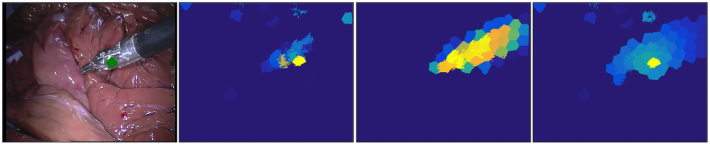
\includegraphics[width=0.99\textwidth]{propagation}
\caption{Probability propagation. Left to right: original image with the gaze location high-
lighted in green; Initial $P_{0}$ estimate from the gaze-based color model; Image regions with high
optical flow; Estimated probability after propagation. Dark blue regions depict low probability
while warmer regions correspond to higher probabilities.}
\label{fig:eel_propagation}
\end{figure}


\section{Experiments}
\label{sec:eel_exp}
To evaluate the performance of our method we compare it to the method presented in \cite{vilarino07}.
We also show how the EEL approach compares with that of using $\epsilon_{S}$ estimates only
(see Sec. \ref{sec:eel_estim}), as well using $\epsilon_{S}$, with a traditional EL when binarizing the labels using a fixed
threshold $\epsilon_{S}=0.5$.
The following parameters were kept constant: $\alpha=0.95$, $\sigma_{a}=0.5$, $\sigma_{d}=50$, $\tau = 50$ and the superpixel size was set to match $\ang{1}$ on the viewing monitor.
We evaluated each of the above mentioned methods on 4 very different image sequences (see
Fig. 1 for examples)

\begin{enumerate}
\item A 3D brain MRI containing a tumor to annotate from the BRATS
challenge \cite{BRATSChall} consisting of 73 slices
\item A 30 frame surgical video sequence from the MICCAI
EndoVision challenge \cite{endochal} where a surgical instrument must be annotated
\item A 95-slice 3D CT scan where a cochlea must be annotated and
\item A slit-lamp video recording (195 frames) of a human retina where the optic disk must be segmented.
\end{enumerate}

Pixel-wise annotated ground truth
on all frames of each sequence was either available or produced by a domain expert.
In all sequences, one and only one object is present throughout the sequence.
Our method was implemented in MATLAB and takes roughly 30 minutes to segment a
30 frame volume with $720 \times 576$ sized frames, of which the bulk of time is used to compute
temporal superpixels and training our classifier.
Even though real-time requirements are not necessary in this application, we believe this computation time could be reduced with an improved implementation.
Gaze locations were collected with an Eye Tribe Tracker (Copenhagen, Denmark) which provide
$\ang{1}$ tracking accuracy.
To collect gaze locations, a computer monitor and the tracker
was placed roughly 1 meter from the experts face.
Device-specific calibration was performed before all recordings (i.e. a 2-minute long procedure done once before each viewing).
2D gaze locations were collected and mapped to the viewed image content using the manufacturers API.
Domain experts were instructed to stare at the target and avoid looking at non-object image
regions.
Once each sequence was observed, the different methods inferred the object throughout
the entire image data.

\section{Results}
\subsection{Annotation accuracy}
Table 1 reports the Area Under the Curve (AUC) and the F1 score performances of each method applied to each dataset.
In general, we report that the proposed combined label estimation and EEL function provide the highest AUC and F1 score values across the tested sequences.
Fig. \ref{fig:eel_qual_res} visually depicts example frames from each sequence and the outcome of each method, as well as the ground truth.

To generate these binary images, a $5\%$ false positive threshold was applied (i.e. threshold was determined using the ground truth).
One can see that in cases where the object to segment occupies large areas of the image,
as is the case for the surgical instrument, both the traditional loss approach and that of \cite{vilarino07} do not perform as well since they treat significant portions of the background as positive samples during their respective learning phases.

\begin{figure}[ht]
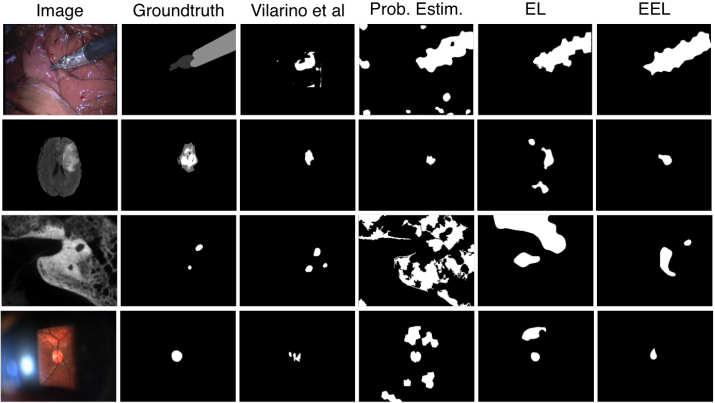
\includegraphics[width=0.99\textwidth]{qual_results}
\caption{Qualitative results. Each row shows a different dataset with an example image,
the associated desired ground truth and the produced outcome of \cite{vilarino07}, using the probability
estimation approach, EL approach and the proposed EEL.
Binary images were generated by thresholding results at a $5\%$ False Positive Rate.}
\label{fig:eel_qual_res}
\end{figure}

\begin{table}
\centering
\caption{Area Under the Curve (AUC) and performances for each approach on each dataset. Highlight maximum values in bold.}
\label{tab:results}
\begin{tabular}{llrrrl}
\toprule
         &    &  Vilarino et al. \cite{vilarino07} &  Probability Est. &     EL &           EEL \\
Type & Metric &                                    &                   &        &               \\
\midrule
\multirow{2}{*}{Brain} & AUC &                              0.687 &             0.963 &  0.974 &  $\bm{0.976}$ \\
         & F1 &                              0.551 &             0.428 &  0.482 &  $\bm{0.592}$ \\
\cline{1-6}
\multirow{2}{*}{Cochlea} & AUC &                              0.687 &             0.963 &  0.974 &  $\bm{0.976}$ \\
         & F1 &                              0.223 &             0.239 &  0.431 &  $\bm{0.631}$ \\
\cline{1-6}
\multirow{2}{*}{Tweezer} & AUC &                              0.346 &             0.949 &  0.959 &  $\bm{0.985}$ \\
         & F1 &                              0.239 &             0.711 &  0.725 &  $\bm{0.851}$ \\
\cline{1-6}
\multirow{2}{*}{Slitlamp} & AUC &                              0.687 &             0.963 &  0.974 &  $\bm{0.976}$ \\
         & F1 &                              0.506 &             0.367 &  0.494 &  $\bm{0.665}$ \\
\bottomrule
\end{tabular}
\end{table}


\subsection{Gaze variance}
In order to estimate the variance in annotations obtained with our strategy, $7$ gaze observations were performed on the same laparoscopic image sequence.
From these gaze observations, we ran our method on each set independently.
Fig. 5(left) shows the average ROC curve and standard error associated with our approach.
In addition, we show similar performances when using the EL and when using the estimated labels only.
On average we see that the EL does no better than the label estimation process, while the label estimation approach has slightly less variability.
Overall, the EEL approach not only outperforms the other settings, but has lower variance as well.

\subsection{Crowd-sourcing context}
From the 7 gaze observations collected, we consider a Crowd-Sourcing context where the label estimation is combined as described in Sec. \ref{sec:eel_estim} in order to generate the associated ground truth.
Fig. 5(right) illustrates the performance attained when doing so.
While the overall trend is no different to the previous experiment, the performance reached by the EEL approach is vastly higher.
This is unsurprising given that more gaze information is provided in this setting (i.e. 7 annotators) and that more of the object is in fact
viewed, yielding thus more positive samples, as well as better $\epsilon_{S}$ estimates.

\begin{figure}[ht]
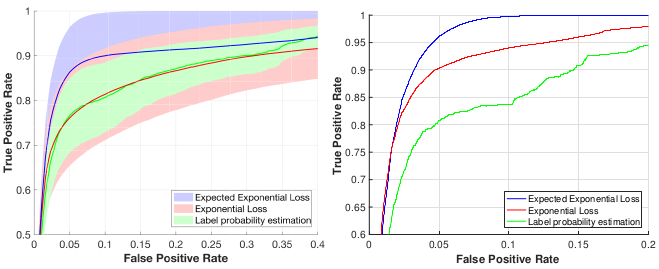
\includegraphics[width=0.99\textwidth]{crowd}
\caption{(left) ROC performance variability on the same data but induced with different gaze
sequences. (right) Performance in a crowd-sourcing setting.}
\label{fig:eel_crowd}
\end{figure}

\section{Conclusion}
In this work we have presented a strategy for domain experts to provide useful pixel-wise
annotations in a passive way. By leveraging cheap eye gaze tracking technology, we have showed
that gaze information can be used to produce segmentation ground truth in a variety of 3D
or video imaging modalities. We achieved this by introducing a novel EEL function that is
robust to large amounts of unlabeled data and few positive samples. We also demonstrated
that our approach could be used in the context of crowd-sourcing where multiple annotators
are available.
While this work presents an initial attempt, a number of aspects of this work need to
be explored moving forward. In particular, we plan to tackle the case when the object is not
present during the entire sequence, as well as cases where multiple objects are present. Naturally,
asking more of the user would provide additional information, but our goal is to keep this to a
minimum. For this reason, we also plan on determining how our method could work with noisy
object observations, as $100\%$ compliant users may not always be possible.
%%% Local Variables:
%%% mode: latex
%%% TeX-master: "../../main"
%%% End:
